\chapter{Interlude --- graph coloring game}

We fix a graph $G$ and a set of colors $C$.

Two players, Alice and Bob, take turns coloring one vertex of $G$ at a time, using a color from $C$, and so that any adjacent vertices which are already colored have different colors. Alice starts. 

Alice wins when all vertices of $G$ are colored (her aim is to color the whole graph). Bob wins if some player has no legal move (he is an adversary trying to stop Alice).

\subsection*{Some games to play}
\medskip

Who has a winning strategy?
\begin{itemize}
\item $G=P_3$, $C=\{1,2\}$
\item $G=P_6$, $C=\{1,2\}$
\item $G=C_6$, $C=\{1,2\}$
\item $G=C_8$, $C=\{1,2,3\}$
\item $G=Q_3$, $C=\{1,2,3,4\}$
\item $G=Q_3$, $C=\{1,2,3\}$
\item $G$ is the tree below, and $C=\{1,2,3\}$
%\begin{center}
%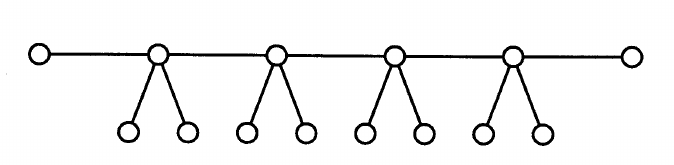
\includegraphics[scale=0.5]{mf4.png}
%\end{center}
\item Come up with your own pair $(G,C)$, where Bob has a winning strategy, and you think this strategy is not easy to find. Play the game instances you came up with against your classmates.
\end{itemize}

\subsection*{Questions}
\medskip
Let $\chi_g(G)$ be the smallest number of colors $k$ for which Alice has a winning strategy in the coloring game on the graph $G$ with $k$ available colors. We call it the \emph{game chromatic number} of $G$.

\begin{itemize}
\item Prove that $\chi(G)\leq \chi_g(G)\leq \Delta(G)+1$.
\item Find bipartite graphs with arbitrarily large $\chi_g$.
\item Describe all graphs with $\chi_g(G)\leq 2$.
\end{itemize}
